\begin{surferPage}[15 cusper]{En flate av femte grad med 15 cusper}
  Denne flaten av femte grad har $15$ singulariteter av typen $A_2$ (kalt cusper). 
  Denne og en rekke relaterte flater ble omtalt i en artikkel fra 2005 av Oliver Labs. 

Fem av spissene ser annerledes ut enn de andre ti. De fem er nemlig singulariteter av 
typen $A_2^{++}$, mens de andre er $A_2^{+-}$ (se galleriet av enkle singulariteter for mer informasjon): 

     \vspace*{-0.3em}
    \begin{center}
      \begin{tabular}{c@{\qquad}c}
        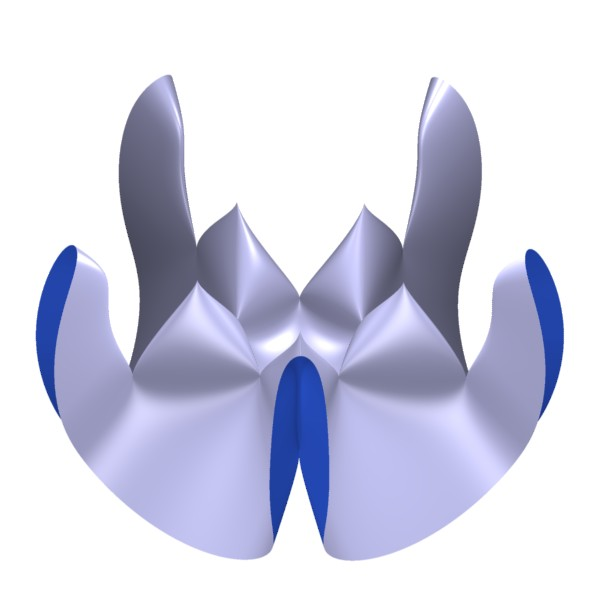
\includegraphics[height=1.2cm]{dessins_quint_15a2}
        &
        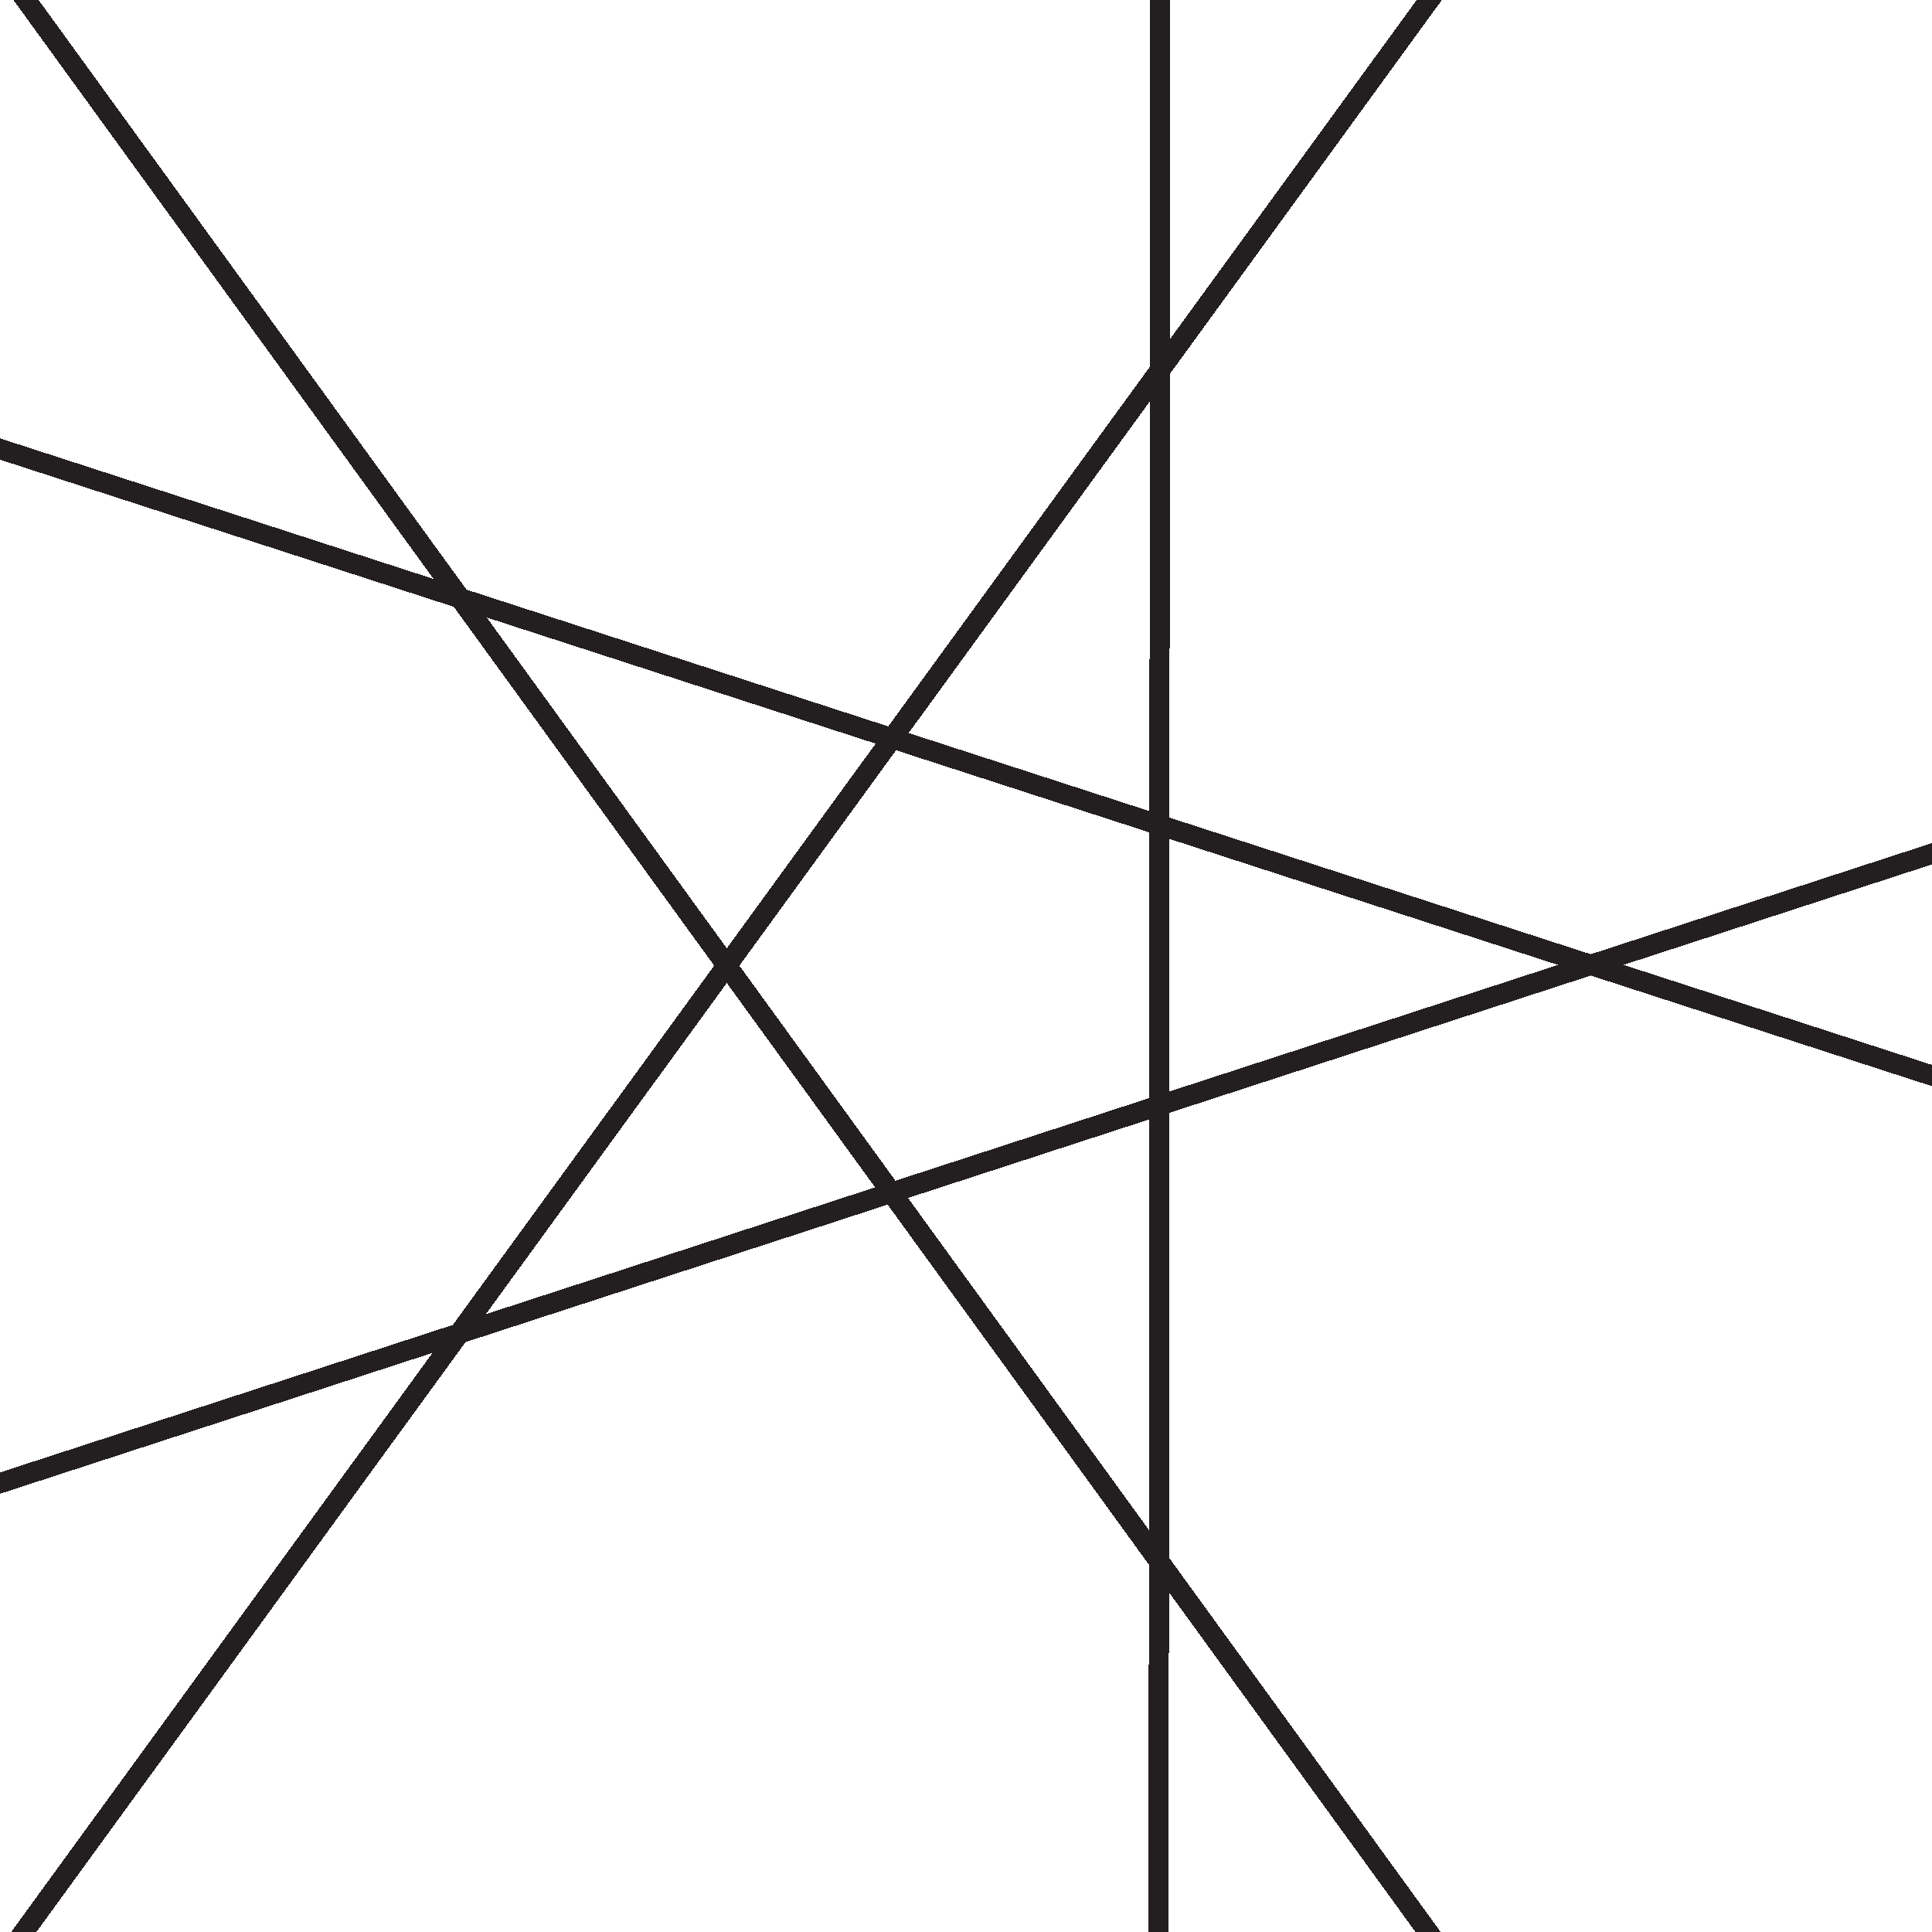
\includegraphics[height=1.2cm]{rp5.pdf}
      \end{tabular}
    \end{center}
    \vspace*{-0.3em}    
    
	Denne flaten har en ligning på formen $S_5(x,y) + t(z)=0$, hvor $S_5(x,y)$ er et vanlig pentagon 
	(bildet til høyre) og $t(z)$ er en variant av Tchebychevs polynomer, som vi har nevnt tidligere. 
    
	
	Wolf Barth konstruerte en annen flate av femte grad med $15$ cusper (se bildet til venstre). 
	Den er relatert til Clebsch-kuben (til høyre), som man kan se fra bildet i midten:


    \vspace*{-0.3em}
    \begin{center}
      \begin{tabular}{c@{\quad}c@{\quad}c}
        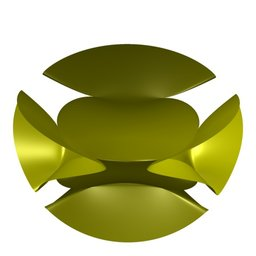
\includegraphics[height=1.2cm]{barthquintic_green}
        &
        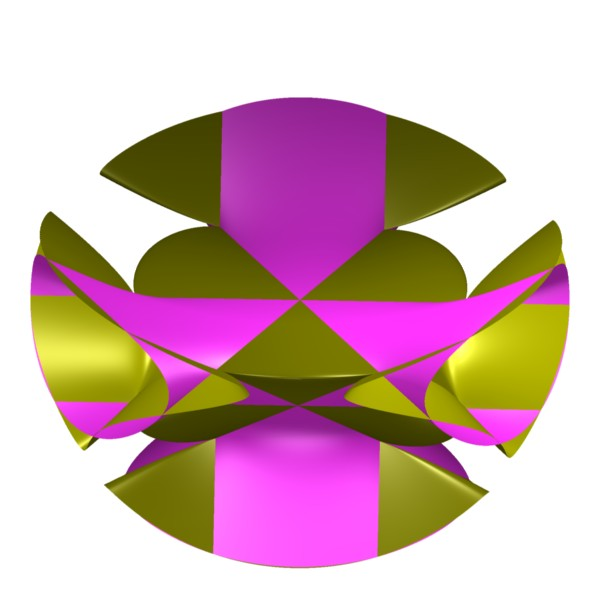
\includegraphics[height=1.2cm]{barthquintic_clebschcubic}
        &
        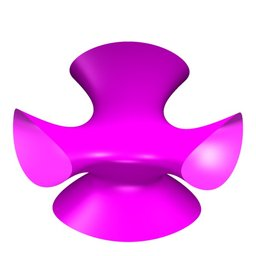
\includegraphics[height=1.2cm]{clebschcubic_pink}
      \end{tabular}
    \end{center}
    \vspace*{-0.3em}
\end{surferPage}
